  %%%%%%%%%%%%%%%%%%%%%%%%%%%%%%%%%%%%%%% -*- coding: utf-8; mode: latex -*- %%
  %
%%%%%                         CHAPTER
 %%%
  %

% $Id: 1020-lorem-ipsum.tex,v 1.2 2009/06/19 15:51:46 david Exp $
% $Log: 1020-lorem-ipsum.tex,v $
% Revision 1.2  2009/06/19 15:51:46  david
% *** empty log message ***
%
% Revision 1.1  2007/11/23 09:52:39  david
% *** empty log message ***
%
%

  %%%%%%%%%%%%%%%%%%%%%%%%%%%%%%%%%%%%%%%%%%%%%%%%%%%%%%%%%%%%%%%%%%%%%%%%%%%%%
  %
%%%%%                           HEAD MATTER
 %%%
  %
\chapter{Evaluation}
\label{ch:evaluation}
\section{Read-Only Nested Snapshots Implementation Evaluation}
%\addcontentsline{lof}{chapter}{\thechapter\quad Lorem Ipsum}
%\addcontentsline{lot}{chapter}{\thechapter\quad Lorem Ipsum}

The algorithm to list subtree of directory at a given snapshot was implemented in SQl and executed against MySql NDB cluster. 
\subsection{Benchmark for measuring query execution time}
In this benchmark, a single directory with 1,000,000 files is used as test directory. Snapshot is taken when vector clock is 5000 i.e after completion 5000 operation. Following operations are executed on the test directory.
\begin{enumerate}
\item \textbf{ADD :} Adding new files to the directory
\item \textbf{DEL:} Deleting exisiting files in the directory
\item \textbf{RENAME:} Renaming exisiting files in the directory
\item \textbf{MOV:} Moving file from this directory to another directory.
\item \textbf{MOV\_ IN:} Moving back the files that were moved out in MOV operation.
\item \textbf{Time:} Time taken for executing listing files in the directory at snapshot taken at time 5000.
These measurements are taken on ndb cluster while the query executed at MySql server instead of clusterj.
\end{enumerate}
\begin{figure*}
\centering  
 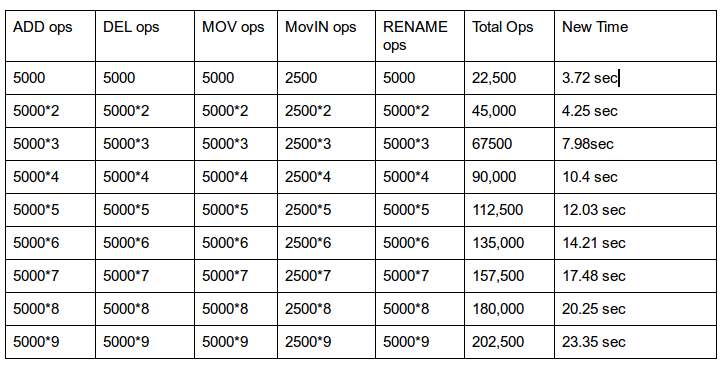
\includegraphics[scale=0.8]{figs/preliminar/Benchmark1.png}
  \caption{Benchmark on Single Directory}
  \label{fig:Benchmark1}
\end{figure*}
\begin{figure*}
\centering  
 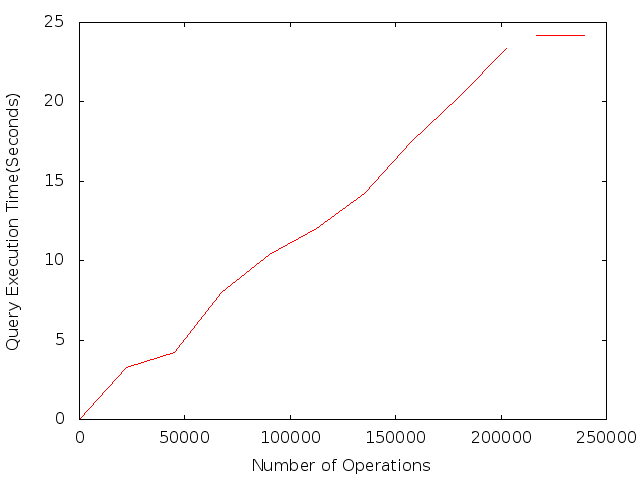
\includegraphics[scale=0.5]{figs/preliminar/benchmark_graph2.png}
  \caption{Benchmark on Single Directory Graph}
  \label{fig:benchmark_graph2}
\end{figure*}

The benchmark\ref{fig:benchmark_graph2} \ref{fig:Benchmark1} shows that the execution time scales linearly with the number of operations. The time to take snapshot is constant which just requires inserting a row into the SNAPS table, where as overhead to take snapshot with the design implemented by Facebook \cite{Facebook} grows linearly \ref{fig:Benchmark_facebook} with the number of files/inodes in the fileSysetm.

\begin{figure*}
\centering  
 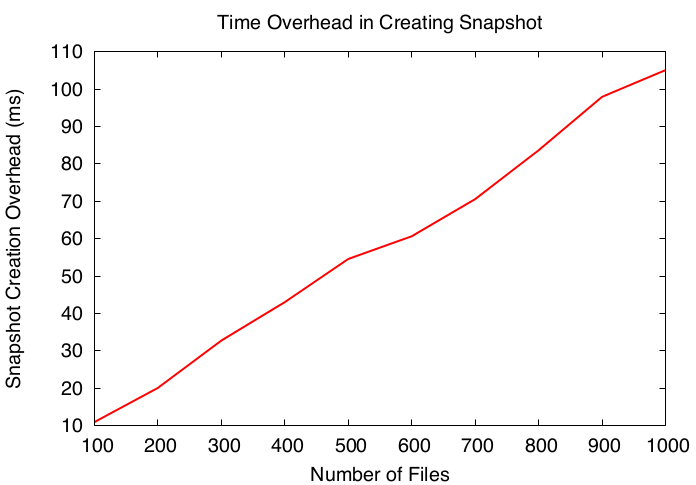
\includegraphics[scale=0.5]{figs/preliminar/Facebook_Snapshots.png}
  \caption{Time Overheads in HDFS@Facebook}
  \label{fig:Benchmark_facebook}
\end{figure*}

\section{Read-Only Root Level Single Snapshot Implementation Evaluation}
\subsection{Evaluation of RollBack}
\textbf{Cluster Configuration}\\
MySql Cluster with 6 data nodes and 1 management server is used for evaluation.The management server which also host mysql server deamon.\\
Management Server\& Data Nodes: 40GB RAM, 24 Intel(R) Xeon(R) CPU X5660  @ 2.80GHz each with 6 Cores.

The roll back algorithm mentioned in \ref{alg:ROSSRB} is implemented using a thread pool, where each thread processes given number of table records [100,000]. The implementation is executed at MySql server as well as via directly connecting NDB-Cluster\cite{29} with ClusterJ\cite{clusterj}. 

The results with evaluation at MySql Server are shown below.\\
\begin{figure*}
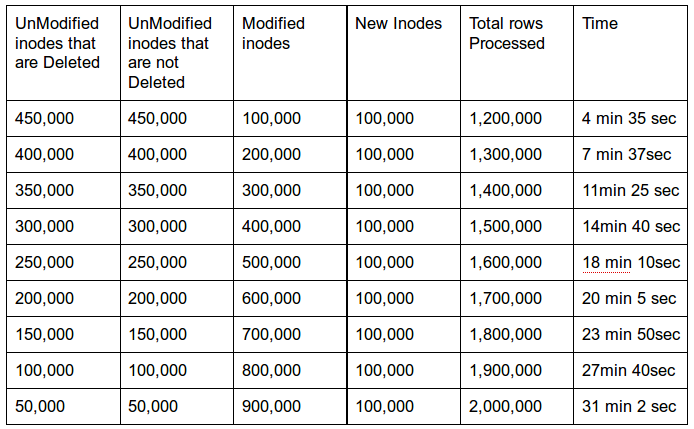
\includegraphics[scale=0.65]{figs/preliminar/MySqlServerSingleSnapshotEval.png}
\captionof{figure}{Benchmark on MySqlServer}\label{fig:MySqlServerSSE}%
\end{figure*}

\pagebreak

\begin{figure*}
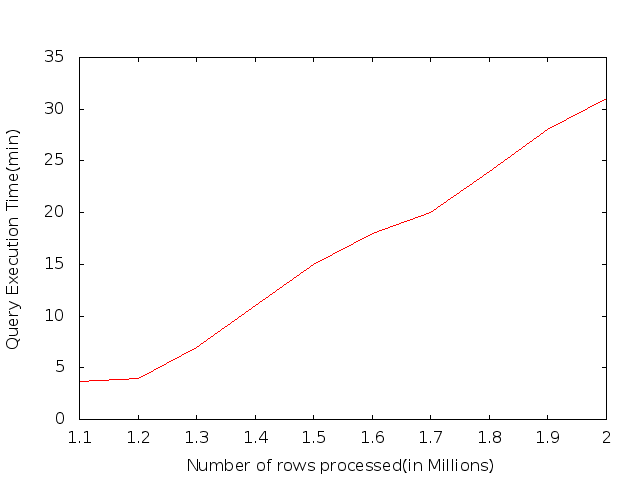
\includegraphics[scale=0.65]{figs/preliminar/MySqlServerSingleSnapshotEvalGraph.png}
\captionof{figure}{Benchmark-Graph on MySqlServer}\label{fig:MySqlServerSSEGraph}%
\end{figure*}

The high execution time with MySql server is because of update of column which is a primary key, in this case id,which we are changing from its negative value to positive value. In evaluations with clusterJ, batch size of rows were read, for each row a new row with id negative of the former row's id is inserted. \\\\
\textbf{Evalaution with ClusterJ}\\
The rollback algorithm explained in section \ref{RollBackImpl} is evalauted with clusteJ and follwing results were obtained.

\begin{figure*}
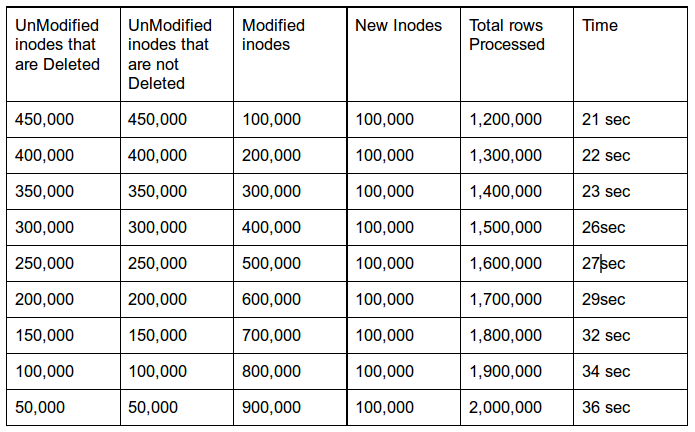
\includegraphics[scale=0.65]{figs/preliminar/ClusterJSingleSnapshotEval.png}
\captionof{figure}{Benchmark with ClusterJ}
\label{fig:ClusterJSSE}%
\end{figure*}

\begin{figure*}
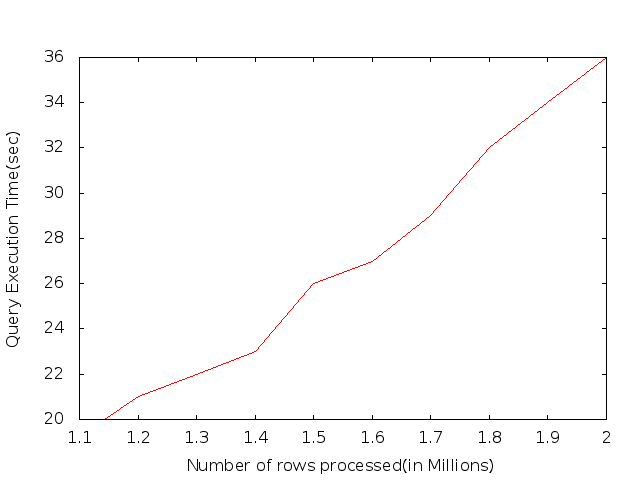
\includegraphics[scale=0.65]{figs/preliminar/benchmark_Clusterj.png}
\captionof{figure}{Benchmark-Graph with ClusterJ}
\label{fig:ClusterJSSEGraph}%
\end{figure*}

As we can infer from above graphs\ref{fig:ClusterJSSEGraph} and \ref{fig:MySqlServerSSEGraph}  that roll-back with clusterJ is efficient and fast.




  %%%%%%%%%%%%%%%%%%%%%%%%%%%%%%%%%%%%%%%%%%%%%%%%%%%%%%%%%%%%%%%%%%%%%%%%%%%%%
  %
%%%%%                        FIRST SECTION
 %%%
  %




  %%%%%%%%%%%%%%%%%%%%%%%%%%%%%%%%%%%%%%%%%%%%%%%%%%%%%%%%%%%%%%%%%%%%%%%%%%%%%
  %
%%%%%                         ANOTHER SECTION
 %%%
  %


  %
 %%%
%%%%%                        THE END
  %
  %%%%%%%%%%%%%%%%%%%%%%%%%%%%%%%%%%%%%%%%%%%%%%%%%%%%%%%%%%%%%%%%%%%%%%%%%%%%%

%%% Local Variables: 
%%% mode: latex
%%% TeX-master: "tese"
%%% End: 
